\documentclass[12pt]{article}

\usepackage[
	top    = 0.50in,
	left   = 1.25in,
	right  = 1.25in,
	bottom = 1.00in,
]{geometry}

\usepackage{amsmath, amssymb, latexsym, xcolor, graphicx, hyperref, tocloft}

\renewcommand \cftsecleader {\cftdotfill 3}
\renewcommand \contentsname {Table of Contents}
\def \combinedDocuments {}

\providecommand \darkMode 1
\ifnum \darkMode = 0 \else
	\pagecolor{black}
	\color[RGB]{170, 170, 170}
\fi

\begin{document}

\title{Physics 1 \& 2 for Engineers (PS 161) – Exam Formulas}
\author{Daniel E. Janusch}
\date{December 10, 2024}
\maketitle

\tableofcontents

\newpage \section{Exam 1 Formulas – Ch. 1-3} % this one might be missing formulas

\ifx \combinedDocuments \undefined
\documentclass[12pt]{article}

\usepackage[
	top    = 0.50in,
	left   = 1.25in,
	right  = 1.25in,
	bottom = 1.00in,
]{geometry}

\usepackage{amsmath, amssymb, latexsym, xcolor}

\providecommand \darkMode 1
\ifnum \darkMode = 0 \else
	\pagecolor{black}
	\color[RGB]{170, 170, 170}
\fi

\begin{document}

\newgeometry{
	top    = 0.00in,
	left   = 1.25in,
	right  = 1.25in,
	bottom = 1.00in,
}

\title{PS 161 Exam 1 Formulas}
\author{Daniel E. Janusch}
\date{December 9, 2024}
\maketitle
\fi

\begin{equation}
	v = v_0 + at
\end{equation}

\begin{equation}
	x = \dfrac{v_0 + v}t
\end{equation}

\begin{equation}
	x = v_0t + \dfrac a2 t^2
\end{equation}

\begin{equation}
	v^2 = v_0^2 + 2 a x
\end{equation}

\begin{equation}
	\text{vector stuff: dot, cross, angle, magnitude}
\end{equation}

\ifx \combinedDocuments \undefined
\end{document}
\fi

\newpage \section{Exam 2 Formulas – Ch. 4-5} % this one might be missing formulas

\ifx \combinedDocuments \undefined
\documentclass[12pt]{article}

\usepackage[
	top    = 0.50in,
	left   = 1.25in,
	right  = 1.25in,
	bottom = 1.00in,
]{geometry}

\usepackage{amsmath, amssymb, latexsym, xcolor}

\definecolor{lightgray}{RGB}{170, 170, 170}
\color{lightgray}
\pagecolor{black}

\begin{document}

\newgeometry{
	top    = 0.00in,
	left   = 1.25in,
	right  = 1.25in,
	bottom = 1.00in,
}

\title{PS 161 Exam 2 Formulas}
\author{Daniel E. Janusch}
\date{December 9, 2024}
\maketitle
\fi

\begin{equation}
	a_c = \dfrac{v^2} r
\end{equation}

\begin{equation}
	f_s = \mu_s N
\end{equation}

\begin{equation}
	f_k = \mu_k N
\end{equation}

\begin{equation}
	a_\parallel = g(\sin \theta - \mu_k \cos \theta) ~~ \text{box sliding down slope}
\end{equation}

\begin{equation}
	F = m a
\end{equation}

\ifx \combinedDocuments \undefined
\end{document}
\fi

\newpage \section{Exam 3 Formulas – Ch. 6-8} \newcommand{\grav}{\textrm{grav}}
\newcommand{\cons}{\textrm{cons}}
\newcommand{\nc}{\textrm{nc}}
\newcommand{\el}{\textrm{el}}
\newcommand{\cm}{\textrm{cm}}
\newcommand{\av}{\textrm{av}}

\newcommand{\pvec}{\hspace{-1px}\vec{\hspace{1px}p}}
\newcommand{\vvec}{\hspace{-1px}\vec{\hspace{1px}v}}

\newcommand{\ds}{\textrm ds}
\newcommand{\dt}{\textrm dt}
\newcommand{\dU}{\textrm dU}
\newcommand{\dW}{\textrm dW}
\newcommand{\dx}{\textrm dx}

\newcommand{\DK}{\Delta K}
\newcommand{\DU}{\Delta U}
\newcommand{\DW}{\Delta W}
\newcommand{\Dy}{\Delta y}
\newcommand{\Dp}{\Delta p}
\newcommand{\Dt}{\Delta t}

\ifx \combinedDocuments \undefined
\documentclass[12pt]{article}

\usepackage[
	top    = 0.5in,
	left   = 1.25in,
	right  = 1.25in,
	bottom = 1.0in,
]{geometry}

\usepackage{amsmath, amssymb, latexsym, xcolor}

\definecolor{lightgray}{RGB}{170, 170, 170}
\color{lightgray}
\pagecolor{black}

\begin{document}

\newgeometry{
	top    = 0.0in,
	left   = 1.25in,
	right  = 1.25in,
	bottom = 1.0in,
}

\title{PS 161 Exam 3 Formulas}
\author{Daniel E. Janusch}
\date{October 22, 2024}
\maketitle
\fi

\begin{equation}
	W = \int_{x_1}^{x_2} \! \vec F \cdot \vec \ds = W_\cons + W_\nc = \DK = \left. \left(\dfrac 12 mv^2~~\text{or}~~\dfrac{p^2}{2m}\right) \right|_{x_1}^{x_2}
\end{equation}

\begin{equation}
	W_F^\cons = -\DU_F
\end{equation}

\begin{equation}
	U_\grav = mgy ~~~~~~~~ U_\el = \dfrac 12 k x^2
\end{equation}

\begin{equation}
	J = \int_{t_1}^{t_2} \! F(t) \,\text dt = \Dp = mv \, \Big|_{t_1}^{t_2} = F_\av\Dt
\end{equation}

\begin{equation}
	F = -\vec \nabla U = \dot{m\vec v}
\end{equation}

\begin{equation}
	P_\av = \dfrac W \Dt ~~~~~~~~ P = \dot W = \vec F \cdot \vvec
\end{equation}

\begin{equation}
	\pvec = m\vvec
\end{equation}

\begin{equation}
	x_\cm = \dfrac{\sum mx}{\sum m} ~~~~~~~~ \vvec_\cm = \dfrac{\sum \pvec}{\sum m}
\end{equation}

\begin{equation}
	\DW = -\DU
\end{equation}

\begin{equation}
	v_{Af},v_{Bf} = \dfrac{p_{Ai} + 2 p_{Bi} - m_B v_{Ai}}{m_A + m_B}, \dfrac{p_{Bi} + 2 p_{Ai} - m_A v_{Bi}}{m_A + m_B}~~(\text{elastic})
\end{equation}

%% Terminal velocity?

\ifx \combinedDocuments \undefined
\end{document}
\fi
\newpage \section{Exam 4 Formulas – Ch. 9-11} 
\providecommand \hpx [1] {\hspace{#1px}}
\providecommand \vpx [1] {\vspace{ #1px}}
\providecommand \nhpx [1] {\hspace{-#1px}}
\providecommand \nvpx [1] {\vspace{-#1px}}

\providecommand \grav {\textrm{grav}}
\providecommand \rad {\textrm{rad}}
\providecommand \rot {\textrm{rot}}
\providecommand \lin {\textrm{lin}}
\providecommand \cm {\textrm{cm}}
\providecommand \cg {\textrm{cg}}
\providecommand \av {\textrm{av}}

\providecommand \pgrp [1] {\left( #1 \right)}

\providecommand \Fvec {\vec F}
\providecommand \pvec {\nhpx 1 \vec {\hpx 1 p}}
\providecommand \rvec {\nhpx 1 \vec {\hpx 1 r}}

\providecommand \dm {\mathrm dm}
\providecommand \dr {\mathrm dr}
\providecommand \DK {\Delta K}

\ifx \combinedDocuments \undefined
\documentclass[12pt]{article}

\usepackage[
	top    = 0.50in,
	left   = 1.25in,
	right  = 1.25in,
	bottom = 1.00in,
]{geometry}

\usepackage{amsmath, amssymb, latexsym, xcolor, graphicx}

\providecommand \darkMode 1
\ifnum \darkMode = 0 \else
	\pagecolor{black}
	\color[RGB]{170, 170, 170}
\fi

\begin{document}

\newgeometry{
	top    = 0.00in,
	left   = 1.25in,
	right  = 1.25in,
	bottom = 1.00in,
}

\title{PS 161 Exam 4 Formulas}
\author{Daniel E. Janusch}
\date{November 12, 2024}
\maketitle
\fi

\begin{equation}
	s = r \theta \hpx{20} v = r \omega \hpx{20} a = r \alpha
\end{equation}

\begin{equation}
	\omega = \omega_0 + \alpha t
\end{equation}

\begin{equation}
	\theta = \omega_\av t = \omega_0 t + \dfrac \alpha 2 t^2
\end{equation}

\begin{equation}
	\omega^2 = \omega_0^2 + 2 \alpha \theta
\end{equation}

\begin{equation}
	a_\rad = \dfrac{v^2}r = r \omega^2
\end{equation}

\begin{equation}
	I = \sum_{i=1}^N m_i r_i^2 = \int \! r^2 \hpx 1 \dm = \int \! r^2 \lambda(r) \dr
\end{equation}

\begin{equation}
	I = I_\cm + m d^2 \Longrightarrow I_2 = I_1 + m \! \pgrp{d_2^2 - d_1^2}
\end{equation}

\begin{equation}
	K_\rot = \dfrac 1 2 I \omega^2
\end{equation}

\begin{equation}
	W = \DK_\lin + \DK_\rot
\end{equation}

\begin{equation}
	U_\grav = m g y_\cm
\end{equation}

\begin{equation}
	\tau = \rvec \times \Fvec = F \ell = F_\perp r = r F \sin \theta = I \alpha = \dot L
\end{equation}

\begin{equation}
	x_\cg = x_\cm ~~~ (\textrm{usually})
\end{equation}

\begin{equation}
	\textrm{statics} \Longrightarrow \sum F = \sum \tau = 0
\end{equation}

\begin{equation}
	\textrm{rolling without slipping} \Longrightarrow v_\cm = r \omega ~~ \land ~~ a_\cm = r \alpha
\end{equation}

\begin{equation}
	P = \tau \omega
\end{equation}

\pagebreak
\restoregeometry

\begin{figure}[ht]
	\centering
	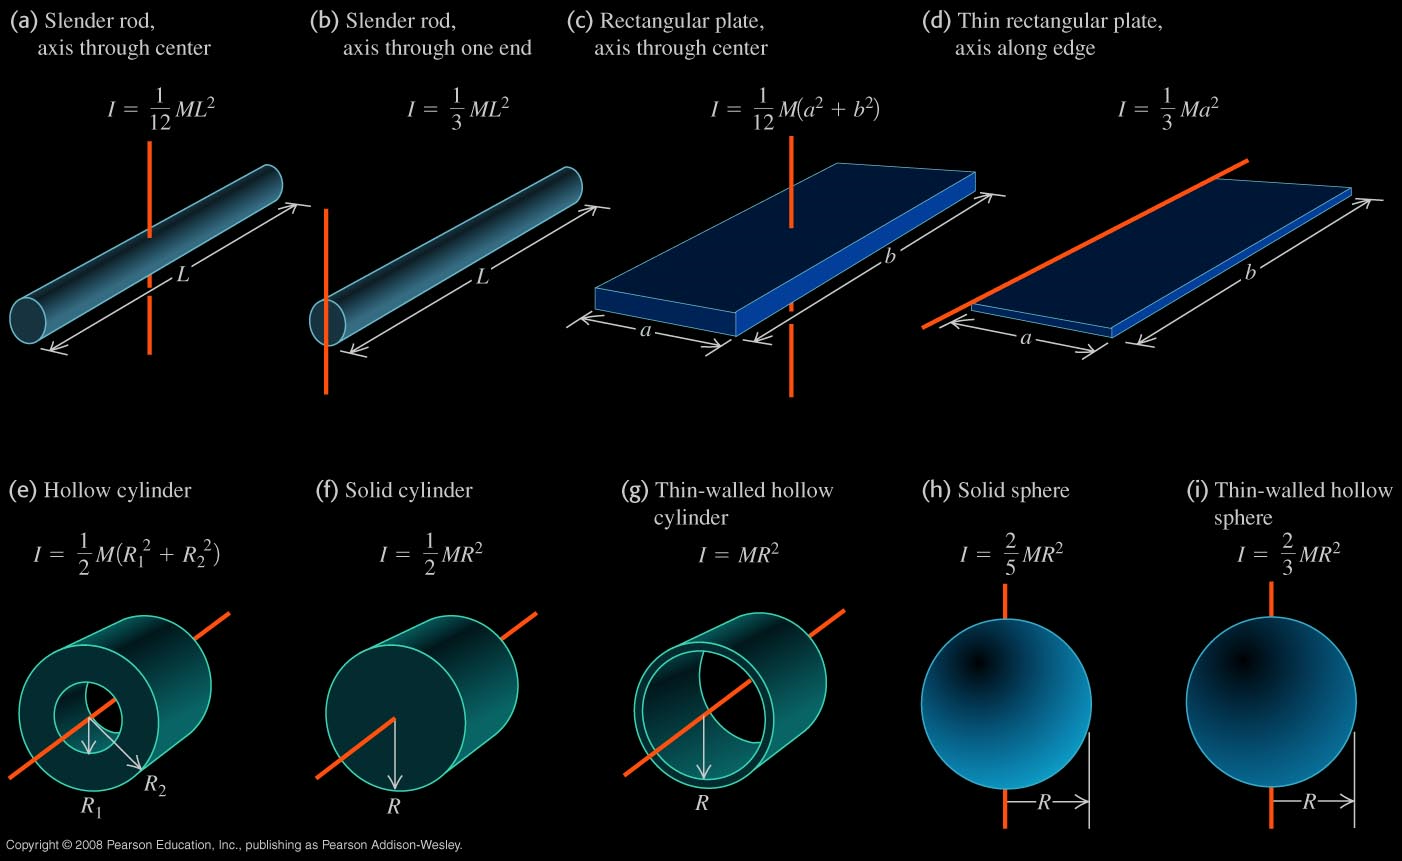
\includegraphics[width=\textwidth]{./rotational-inertia-table.png}
\end{figure}

\nvpx{20} \begin{equation}
	L = \rvec \times \pvec = mvr \sin \theta = mv\ell = I \omega
\end{equation}

\begin{equation}
	\hpx{36} L_0 = L_1 ~~~~ (\textrm{assuming no external torque})
\end{equation}

% \begin{equation}
% 	\Omega = \dot \phi = \dfrac \tau L = \dfrac{w r} {I \omega} ~~~~~ (\textrm{gyroscope})
% \end{equation}

% \begin{equation}
% 	\tau = \rvec_\cm \times \wvec
% \end{equation}

\ifx \combinedDocuments \undefined
\end{document}
\fi
\newpage \section{Final Exam Formulas – Ch. 12-14} \ifx \combinedDocuments \undefined
\documentclass[12pt]{article}

\usepackage[
	top    = 0.50in,
	left   = 1.25in,
	right  = 1.25in,
	bottom = 1.00in,
]{geometry}

\usepackage{amsmath, amssymb, latexsym, xcolor, graphicx}

\definecolor{lightgray}{RGB}{170, 170, 170}
\color{lightgray}
\pagecolor{black}

\begin{document}

\newgeometry{
	top    = 0.00in,
	left   = 1.25in,
	right  = 1.25in,
	bottom = 1.00in,
}

\title{PS 161 Final Exam Formulas}
\author{Daniel E. Janusch}
\date{December 9, 2024}
\maketitle
\fi

\begin{equation}
	\lambda = \dfrac mL ~~~~~~~~~~
	\sigma = \dfrac mA ~~~~~~~~~~
	\rho = \dfrac mV
\end{equation}

\begin{equation}
	p = \rho g h = \dfrac{F_1}{A_1} = \dfrac{F_1}{A_2}~~[\text{Pa}]
\end{equation}

\begin{equation}
	F_{\text{pressure}} = p A
\end{equation}

\begin{equation}
	F_{\text{buoyant}} = \rho g V
\end{equation}

\begin{equation}
	R = A v~~(\text{flow rate})
\end{equation}

\begin{equation}
	\rho_1 R_1 = \rho_2 R_2~~(\text{mass flux})
\end{equation}

\begin{equation}
	\rho_1 = \rho_2~~(\text{incompressible})
\end{equation}

\begin{equation}
	M\!E = p + \dfrac 12 \rho v^2 + \rho g y
\end{equation}

\begin{equation}
	U_g = -\dfrac{GMm} r
\end{equation}

\begin{equation}
	F_g = -\dfrac{GMm}{r^2}
\end{equation}

\begin{equation}
	v_{\text{orbit}} = \sqrt{\dfrac{GM}{R}}
\end{equation}

\begin{equation}
	v_{\text{escape}} = v_{\text{orbit}} \sqrt 2
\end{equation}

\begin{equation}
	T = \dfrac{2 \pi r}v = \dfrac{2 \pi r^{1.5}}{\sqrt{G M}}
\end{equation}

\begin{equation}
	R_S = \dfrac{2 G M}{c^2}
\end{equation}

\pagebreak
\restoregeometry

Simple Harmonic Motion (SHM):
\begin{equation}
	x(t) = A \cos(\omega t + \phi) \ni \omega^2 = \dfrac k m
\end{equation}

\begin{equation}
	\omega = 2 \pi f
\end{equation}

\begin{equation}
	E = \dfrac{m v^2 + k x^2}2
\end{equation}

\begin{equation}
	v = \pm \omega \sqrt{A^2 - x^2}
\end{equation}

\begin{equation}
	\theta(t) = \theta_0 \cos(\omega t + \phi)
\end{equation}

\begin{equation}
	\text{Angular SHM: } \omega^2 = \dfrac \kappa I \ni \kappa = \text{torsion constant}
\end{equation}

\begin{equation}
	\text{Small $\theta$ Simple Pendulum: } \omega^2 = \dfrac g L
\end{equation}

\begin{equation}
	\text{Physical Pendulum: } \omega^2 = \dfrac {mgd} I
\end{equation}

\ifx \combinedDocuments \undefined
\end{document}
\fi


\end{document}
